\chapter{Bornholdt model}\label{ch:chapter2}
We now present the model proposed in \cite{bornholdt}. The idea is to formulate a model with maximum simplicity, which includes the possibility of strategic interaction in the market. The model is based on the Ising model, which is a model of ferromagnetism in statistical mechanics.

\section{Theoretical background: the Ising model}
The Ising model is a simple mathematical model of ferromagnetic materials. In its description, we will mostly follow the notation and tools presented in \cite{mezard_book} and from professor Mézard's lecture notes. The model consists of Ising spins (that is, spins which can take binary values) on a d-dimensional cubic lattice (see figure \ref{fig:ising_model}). Mathematically, given a cubic lattice $\mathbb{L}=\{1,\dots,L\}^n$, we define an an Ising spin $\sigma_i\in\{-1,1\}$ for each site $i\in\mathbb{L}$. Then, we can have any configuration $\underline{\sigma} = (\sigma_1,\dots,\sigma_n) \in \mathcal{X}_N=\{+1,-1\}^{\mathbb{L}}$.

\begin{figure}[h]
    \centering
    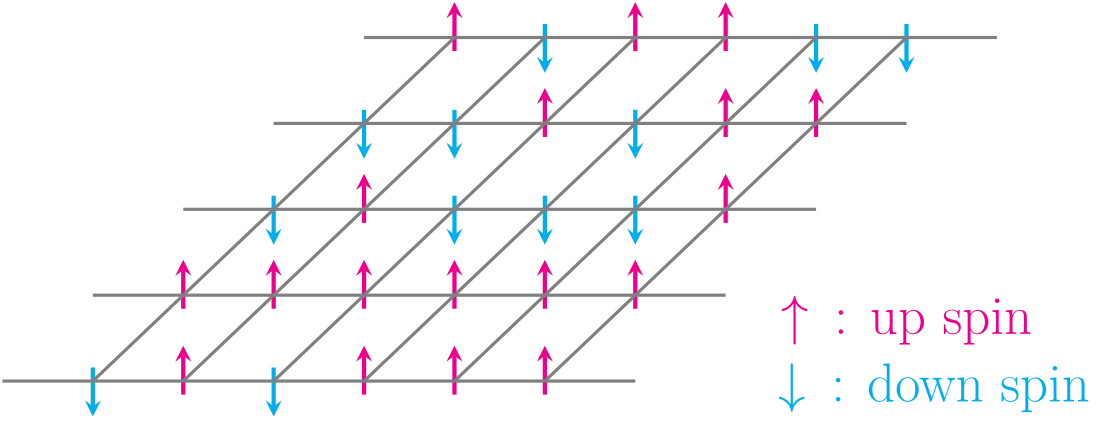
\includegraphics[width=0.5\textwidth]{2D_ising_model_on_lattice.svg.png}
    \caption{The Ising model on a 2D lattice.}
    \label{fig:ising_model}
\end{figure}


The energy of a configuration $\underline{\sigma}$ is given by:
\begin{equation}
    H(\underline{\sigma}) = -\sum_{\langle i,j\rangle}\sigma_i\sigma_j - B\sum_i \sigma_i
\end{equation}
Where the sum over $\langle i,j\rangle$ is a sum over all nearest neighbors, and $B$ is an external magnetic field. At equilibrium, the probability of a configuration $\underline{\sigma}$ is given by the Boltzmann distribution:
\begin{equation}
    P(\underline{\sigma}) = \frac{e^{-\beta H(\underline{\sigma})}}{Z}
\end{equation}
Where $\beta$ is the inverse temperature, and $Z$ is the partition function:
\begin{equation}
    Z = \sum_{\underline{\sigma}\in\mathcal{X}_N}e^{-\beta H(\underline{\sigma})}
\end{equation}
Interestingly, despite its simplicity, an analytical solution has been found only in the $d=1$ and $d=2$ cases. Higher dimensions remain unsolved, but numerical methods and mean-field approximations can be used to study the model in these cases.

One important quantity in the Ising model is the magnetization, which is defined as:
\begin{equation}
    m = \frac{1}{N}\sum_i \langle \sigma_i \rangle
\end{equation}
where $\langle \cdot \rangle$ denotes the average.

\subsection{Solution of the Ising model in the one-dimensional case}
For simplicity, assume $B=0$. In the one-dimensional case, the Ising model can be solved exactly. Recall that:
\begin{equation}
    H(\underline{\sigma}) = -\sum_{\langle i,j\rangle}\sigma_i\sigma_j
\end{equation}
Then, the partition function is given by:
\begin{equation}
    Z = \sum_{\underline{\sigma}\in\mathcal{X}_N}e^{-\beta H(\underline{\sigma})} =
    \sum_{\underline{\sigma}\in\mathcal{X}_N}e^{\beta\sum_{\langle i,j\rangle}\sigma_i\sigma_j}
\end{equation}
Since each spin is connected to its nearest neighbors, we can write:
\begin{equation}
    Z =  \sum_{\underline{\sigma}\in\mathcal{X}_N}e^{\beta\sum_n\sigma_n\sigma_{n+1}}
\end{equation}
Let us define $\tau_n = \sigma_{n-1}\sigma_{n} \implies \sigma_n = \tau_n\tau_{n-1}\dots\tau_2\sigma_1$. Then, we can write:
\begin{equation}
    \begin{gathered}
    Z =  \sum_{\sigma_1\in\{-1,1\}}\sum_{\tau_2,\dots\tau_n}e^{\beta\sum_n\tau_n}
    = 2\sum_{\tau_2,\dots,\tau_N}e^{\beta\sum_n\tau_n}\\
    = 2\sum_{\tau_2,\dots,\tau_N}\prod_n e^{\beta\tau_n}
    = 2(\sum_{\tau_2}e^{\beta\tau_2})\dots(\sum_{\tau_N}e^{\beta\tau_N})\\
    = 2(2\cosh(\beta))^{N}
    \end{gathered}
\end{equation}
Thus, we have found an analytical expression for the partition function in the one-dimensional case. The magnetization can be computed as:
\begin{equation}
    m = \frac{1}{N}\sum_i \langle \sigma_i \rangle = \frac{1}{N}\frac{\partial}{\partial \beta}\log Z = \tanh(\beta)
\end{equation}
%check magnetization formula

% \subsection{The Curie-Weiss model}
% The Curie-Weiss model is remarkably similar to the Ising model, but with all the spins interacting with each other, then, the model represents a fully connected graph of spins rather than a lattice. The Hamiltonian is given by:
% \begin{equation}
%     H(\underline{\sigma}) = -\frac{1}{N}\sum_{i,j}\sigma_i\sigma_j - B\sum_i \sigma_i
% \end{equation}
% The scaling factor $\frac{1}{N}$ is introduced to have a non-trivial free energy. This model is interesting because it introduced the concept of mean-field approximations. To compute the partition function, we first notice that the empirical magnetization is:
% \begin{equation}
%     m(\underline{\sigma}) = \frac{1}{N}\sum_i  \sigma_i
% \end{equation}
% Then, we can write:
% \begin{equation}
%     H(\underline{\sigma}) = \frac{1}{2}N- \frac{1}{2}N m(\underline{\sigma})^2 - NB m(\underline{\sigma})
% \end{equation}




\subsection{Mean-field approximation of the Ising model in higher dimensions}
While a closed-form solution for the Ising model in two dimensions exists, it does not for $d\geq 3$ so we will study its mean-field approximation. The method we will see can be applied to a more general Ising model, and then be reconduced to the original one. The hamiltonian we focus on is:
\begin{equation}
    H(\underline{\sigma}) = -\sum_{\langle i,j\rangle}J_{i,j}\sigma_i\sigma_j - \sum_i B_i\sigma_i
\end{equation}
Which differs from the standard Ising model by having arbitrary $J_{i,j}$ and $B_i$ for every $i,j$. The idea is to approzimate the Boltzmann distribution $P(\underline{\sigma}) = (1/Z)e^{-\beta H(\underline{\sigma})}$ with a probability with independent variables $Q(\underline{\sigma})= \prod_{i=1}^Nq_i(\sigma_i)$. The idea is to find the $q_i$ such that the ``distance'' between $P$ and $Q$ is minimized. We will use the Kullback-Leibler divergence as notion of distance.
\begin{definition}
    Given $p(x)$ and $q(x)$ probability distributions over the same finite space $\mathcal{X}$, the Kullback–Leibler (KL) divergence between them is:
    $$D(q||p) = \sum_{x\in\mathcal{X}}q(x)\log\frac{q(x)}{p(x)}$$
\end{definition}
\begin{remark}
    \hfill
    \begin{enumerate}
        \item $D(q||p)$ is convex in $q(x)$.
        \item $D(q||p)\geq 0$ with equality $ \iff p(x)=q(x) \;\forall x\in\mathcal{X}$.
        \item In general, the KL divergence is not symmetric.
    \end{enumerate}
    Then, the KL divergence lacks the symmetry property to be properly defined as a distance between probability distributions.
\end{remark}
We will define $Q$ as the most general joint binary probability distribution:
\begin{equation}
    Q(\underline{\sigma}) = \prod_{i=1}^{N}q_i(\sigma_i); \quad
    q_i(\sigma_i)=\frac{1+m_i\sigma_i}{2}
\end{equation}
Where $m_i$ is the mean of each $q_i$, and it is the parameter which we want to find. Then,
\begin{equation}
    \begin{gathered}
        D(Q||P) = \sum_{\underline{\sigma}\in\mathcal{X}}Q(\underline{\sigma})\log\frac{Q(\underline{\sigma})}{P(\underline{\sigma})}\\
        =\sum_{\underline{\sigma}\in\mathcal{X}}Q(\underline{\sigma})\log Q(\underline{\sigma}) - \sum_{\underline{\sigma}\in\mathcal{X}}Q(\underline{\sigma})\log P(\underline{\sigma}) = (A) + (B)\\
    \end{gathered}
\end{equation}
We can split this in the first term, depending only on $Q$, and the second term, depending on $P$ as well. Then:
\begin{equation}
    \begin{gathered}
        (A) = \sum_{\underline{\sigma}\in\mathcal{X}}Q(\underline{\sigma})\log Q(\underline{\sigma}) = \sum_{i=1}^{N}\left(\frac{1+m_i}{2} \log \frac{1+m_i}{2}+\frac{1-m_i}{2} \log \frac{1-m_i}{2}\right)\\
        (B) = \beta \sum_{i<j} J_{i j} m_i m_j + \beta \sum_i B_i m_i-\log Z
    \end{gathered}
\end{equation}
In the second term, we see that the $\log Z$ term is independent of $m_i$, so we can ignore it. Then, we are interested in finding the values of $m_i$ that solve:
\begin{equation}
    \frac{\partial D(Q||P)}{\partial m_i} = 0 \iff \frac{1}{2} \log \frac{1+m_i}{1-m_i} - \beta \sum_{j\in \partial_i} J_{i j} m_j - \beta B_i = 0
\end{equation}
Then, we find the mean field equation:
\begin{equation}
    m_i = \tanh\left(\beta\sum_{j\in \partial_i} J_{i j} m_j + \beta B_i\right)
\end{equation}
Now, going back to the original Ising model, we can set $J_{i,j} = J$ and $B_i=B \implies m_i = m$. Then, we have the mean field equation for the Ising model in $d$ dimensions:
\begin{equation}
    m = \tanh(\beta (B + 2dJm))
\end{equation}
Let us consider the case $B=0$. Then, depending on the value of $\beta$, we can have one or three solutions to the mean-field equation, depending on the slope of the function $f(m) = \tanh(\beta 2dJm)$. The critical value of $\beta$ is then:
\begin{equation}
    \beta_c = \frac{1}{2dJ}
\end{equation}

\subsection{The Curie-Weiss model}
\textcolor{red}{TBA: definition and mean-field approximation of the curie weiss model}

\section{Financial background: option pricing}
\label{sec:financial_background}
\textcolor{red}{TBA: introduction}
\subsection{Setting and options}
Let $\mathcal{T}$ be the set of trading times, and let $\Omega$ be the state space of the price of a stock. Let $\mathcal{P} = \{\mathcal{P}_t\}_{t\in\mathcal{T}}$ be a filtration on $\Omega$. On this setting, we can define a locally riskless asset $\{B(t)\}_{t\in\mathcal{T}}$, described by a $\mathcal{P}_t$-measurable stochastic process $\{r(t)\}_{t\in\mathcal{T}}$, which is the return of $B(t)$ at time $t$. The return is defined as:
\begin{equation}
    r(t) = \frac{B(t+1)-B(t)}{B(t)} \quad \forall t\in\mathcal{T}
\end{equation}
We can also define N risky asset as $\mathcal{P}_{t+1}$-measurable stochastic processes $\{S_i(t)\}_{t\in\mathcal{T}} \; i\in \{1,\dots,N\}$, which is the price of each asset at time $t$. Intuitively, the locally riskless asset is a bond, for which we know the return at time $t+1$ given the return at time $t$. The risky assets are stocks, for which we do not know the return at time $t+1$ given the return at time $t$.

Let $\theta_j = \{\theta_j(t)\}_{t\in\mathcal{T}}$ be stochastic process representing the value of the position held in the j-th asset, which might be positive or negative (in the case of short selling).

We can now go ahead and define what a european call option is.
\begin{definition}
    A european call option is a contract that gives the holder the right, but not the obligation, to buy an asset at a specified price (the strike price) at a specified time (the expiration date). The payoff of a european call option at time $t$ is given by:
    \begin{equation}
        X(t) = \begin{cases}
            max(S(t)-K,0) & \text{if } t = T\\
            0 & \text{if } t < T
        \end{cases}
    \end{equation}
    Where $S(t)$ is the price of the underlying asset at time $t$, $K$ is the strike price, and $T$ is the expiration date. The payoff is zero if the option is not exercised, and it is equal to the difference between the price of the underlying asset and the strike price if the option is exercised.
\end{definition}

A european put option is defined similarly, but it is defined as the right to sell an asset at a specified price at a specified time.

\subsection{Assumptions of the Black-Scholes model}
The Black-Scholes model is a mathematical model for the pricing of european options, indtroduced in \cite{black_scholes}. The assmuptions for deriving the price of the option are:
\begin{enumerate}
    \item The locally riskless asset is known and constant over time: $r(t) = r \;\forall t\in\mathcal{T}$.
    \item  \label{it:gbm}The risky asset follows a geometric Brownian motion, meaning that the price of the asset at time $t$ is given by:
    \begin{equation}
        S(t) = S(0)e^{(r-\frac{\sigma^2}{2})t+\sigma W(t)}
    \end{equation}
    \textcolor{red}{TBA: check this equation}
    Where $W(t)$ is a standard Brownian motion, and $\sigma$ is the volatility of the asset.
    \item The market is frictionless, meaning that there are no transaction costs, and the assets can be traded continuously.
    \item The asset pays no dividends.
    \item It is possible to short-sell the asset without any restrictions or penalties.
    \item It is possible to borrow a fraction of the security at the risk-free rate.
\end{enumerate}
\textcolor{red}{TBA: Black-Scholes model (if deemed useful)}\\
This model is widely used in the financial industry, and it is the basis for many other models. \textcolor{red}{part about how useful the model is and how important derivatives are}
The key assumption of this model is \ref{it:gbm}, which requires that the price of the underlying asset follows a geometric Brownian motion. This would imply that the distribution of prices in any finite period is log-normal. This assumption has more to do with the ease of computation that such a distribution allows rather than the real-world features of financial data. As a matter of fact, it has been shown that the distribution of returns is fat-tailed, meaning that there are more extreme events than would be predicted by a normal distribution, and the returns show autocorrelation, which means that returns are not independent over time. This is a key observation, and it is one of the main motivations for studying models such as the Bornholdt model.

\section{The Bornholdt model}
\subsection{Financial motivation}
In \cite{bornholdt}, a simple spin model, which we will refer to as the Bornholdt model, is proposed to model trading in financial markets. In the model, agents are seen as interacting spins, which have two possible actions: buy or sell an asset. The choice of each agent is influenced by two contrasting forces:
\begin{itemize}
    \item ``Do what your neighbors do'': this is the strategy that momentum traders follow. They try to follow the trend in the market, buying when the price is rising and selling when it is falling.
    \item ``Do what the minority does'': this is the strategy that mean-reversion traders follow. They try to buy when the price is falling and sell when it is rising, betting on a reversal of the trend.
\end{itemize}
We will see how these two strategies are implemented in the model.

\subsection{Model definition}
Consider a model with N spins with orientations $\sigma_i\in\{-1,+1\}$, representing the decision of agent $i$ to buy or sell a stock. We will consider updates following a heat-bath dynamics:
\begin{equation}
    \begin{aligned}
        \sigma_i(t+1) &= +1 \;\text{with }\; p = \frac{1}{1+e^{-2\beta h_i(t)}}\\
        \sigma_i(t+1) &= -1 \;\text{with }\; 1-p
    \end{aligned}
    \label{eq:heat_bath}
\end{equation}
Where $h_i(t)$ is the local field of agent $i$ at time $t$:
\begin{equation}
    h_i(t)=\sum_{j=1}^N J_{i j} \sigma_j-\alpha C_i(t) \frac{1}{N} \sum_{j=1}^N \sigma_j(t)
\end{equation}
Where $J_{i j}$ is the coupling between agents $i$ and $j$, $\sigma_j$ is the agent's action at $t$, $C_i(t)$ is the strategy of $i$ at time $t$, and $\alpha$ is a parameter. The first term in the local field pushes the agent to follow the trend (do what your neighbors do), while the second term pushes the agent to follow the minority (do what the minority does), assuming the strategy $C_i(t)$ is positive. 
If we consider the case in which $C_i(t) = 1\;\forall i, t$, we have that each trader follows both a momentum and a mean-reversion strategy simultaneously. This leads to near-vanishing magnetization even for temperatures below the critical temperature. We will focus on the more interesting case in which the strategy is updated according to:
\begin{equation}
    C_i(t+1) = -C_i(t) \quad\text{if} \; \alpha\sigma_i(t)C_i(t) \sum_{j=1}^N \sigma_j(t)< 0
\end{equation}
When we assume the strategy adjustment to be done instantaneously, we can write the local field as:
\begin{equation}
    h_i=\sum_{j=1}^N J_{i j} \sigma_j-\alpha \sigma_i \left | \frac{1}{N}\sum_{j=1}^N \sigma_j \right |
\end{equation}
Then, the hamiltonian of the model is:
\begin{equation}
    H(\underline{\sigma}) = \sum_{i,j}J_{i,j}\sigma_i\sigma_j - \frac{\alpha}{N}\sum_{i=1} \sigma_i \left | \sum_{j=1}^N \sigma_j \right |
\end{equation}
Then, the magnetization \(M = \frac{1}{N}\sum_{j=1}^N \sigma_j\) can be interpreted as the price of the security that is being traded. We seek to study the dynamics of the model.

\subsection{Analysis of the model}
We will focus on the fully connected case in which \(J_{i,j}=\frac{J}{N} \; \forall i,j\). The hamiltonian of the model is then:
\begin{equation}
    H(\underline{\sigma}) = \frac{J}{N}\sum_{i,j}\sigma_i\sigma_j - \frac{\alpha}{N}\sum_{i=1} \sigma_i \left | \sum_{j=1}^N \sigma_j \right |
\end{equation}

\textcolor{red}{TBA: Analysis of the model}
